\documentclass{article}
\usepackage[utf8]{inputenc}
\usepackage[english]{babel}
\usepackage{biblatex}
\usepackage{amsmath}
\usepackage{amssymb}
\usepackage{caption}
\usepackage{subcaption}
\usepackage{graphicx}
\usepackage{csquotes}
\usepackage{booktabs}
\usepackage{lipsum}
\usepackage{setspace}
\usepackage[letterpaper,top=2cm,bottom=2cm,left=3cm,right=3cm,marginparwidth=1.75cm]{geometry}
\usepackage{amsthm}

% Font
\usepackage{charter}

% Hyperlink config
\usepackage{hyperref}
\hypersetup{
    colorlinks=true,
    linkcolor=blue,
    filecolor=magenta,      
    urlcolor=cyan,
    pdftitle={Overleaf Example},
    pdfpagemode=FullScreen,
}

% Code snippets
% \usepackage{minted}
\usepackage{minted}
\usepackage{xcolor}
\usepackage{caption}

\definecolor{codebg}{rgb}{0.95,0.95,0.95}
\definecolor{codeframe}{rgb}{0.75,0.75,0.75}

% Title and footnote
\usepackage{titling}
\newcommand{\subtitle}[1]{%
  \posttitle{%
    \par\end{center}
    \begin{center}\large#1\end{center}
    \vskip0.5em}%
}
\usepackage{hyperref}
\newcommand{\footremember}[2]{%
   \footnote{#2}
    \newcounter{#1}
    \setcounter{#1}{\value{footnote}}%
}

\renewcommand{\baselinestretch}{1.15}
\addbibresource{ref.bib}

\setlength{\parindent}{0em}
\setlength{\parskip}{0.5em}

\title{CS 5785 Homework 3}
\subtitle{Cornell Tech}

\author{
    Tian Jin\thanks{Both authors contributed equally to this project.} \thanks{\href{mailto:tj299@cornell.edu}{tj299@cornell.edu}}
    \and 
    Yufan Zhang\footnotemark[1] \thanks{\href{mailto:yz2894@cornell.edu}{yz2894@cornell.edu}}
}

\date{October 2023}


% ======================
\begin{document}

\maketitle

\section{Programming Exercises}
\subsection{Eigenface for face recognition}

\subsection{Implement EM algorithm}

\subsection{Kernel Density Estimation}

\subsubsection*{Part (a) Plot the density estimate}

We are given the following data: 

\[26, 30, 27, 18, 75, 66, 73, 63, 56, 83\]

Before implementing and plotting the kernel density estimate (KDE) of the given dataset, we need to first use the code in Listing~\ref{code:kde_prepare} to prepare our data and the range of $x$ values for plotting.

\begin{listing}[H]
\caption{Prepare the data, bandwidths, and x value for plottting}
\label{code:kde_prepare}
\begin{minted}[bgcolor=codebg, frame=lines, framesep=2mm, linenos]{python}
# Given data
data = np.array([26, 30, 27, 18, 75, 66, 73, 63, 56, 83]).reshape(-1, 1)

# Bandwidths to use
bandwidths = [100, 10]

# Range of x values for plotting
x_vals = np.linspace(min(data)-20, max(data)+20, 1000).reshape(-1, 1)
\end{minted}
\end{listing}

Listing~\ref{code:kde_sklearn} shows the code to plot the KDE of the given dataset using a Gaussian kernel with Sklearn.

\begin{listing}[H]
\caption{Plot the kernel density estimate (KDE) using a Gaussian kernel with Sklearn}
\label{code:kde_sklearn}
\begin{minted}[bgcolor=codebg, frame=lines, framesep=2mm, linenos]{python}
from sklearn.neighbors import KernelDensity

# Plotting using sklearn
plt.figure(figsize=(10, 5))
for bandwidth in bandwidths:
    kde = KernelDensity(kernel='gaussian', bandwidth=bandwidth).fit(data)
    log_dens = kde.score_samples(x_vals)
    plt.plot(x_vals, np.exp(log_dens), label=f'$\delta$ = {bandwidth}')

plt.title('Kernel Density Estimate using sklearn')
plt.legend()
plt.xlabel('x')
plt.ylabel('Density')
plt.grid(True)
plt.show()
\end{minted}
\end{listing}

Moreover, we manually implement the KDE using NumPy and plot the density estimates. The formula for the KDE with a Gaussian kernel is:

\[
\tilde{p}(x) = \frac{1}{n\delta} \sum_{i=1}^{n} K\left(\frac{x - x_i}{\delta}\right)
\]

where

\[
K(u) = \frac{1}{\sqrt{2\pi}} e^{-\frac{u^2}{2}}
\]


Listing~\ref{code:kde_sklearn} shows the code to plot the KDE of the given dataset using a Gaussian kernel, manually calculated with bandwidth parameters \( \delta = 100 \) and \( \delta = 10 \).

Figure~\ref{fig:kde_plot} illustrates the kernel density estimate of the given dataset using a Gaussian kernel, as computed by the \texttt{sklearn} library and manual implementation with bandwidth parameters \( \delta = 100 \) and \( \delta = 10 \). The results are consistent between these two implementations.

\begin{listing}[H]
\caption{Plot the kernel density estimate (KDE) using a Gaussian kernel with manual implementation}
\label{code:kde_manual}
\begin{minted}[bgcolor=codebg, frame=lines, framesep=2mm, linenos]{python}
# Defining the Gaussian kernel function
def gaussian_kernel(u):
    return (1/np.sqrt(2*np.pi)) * np.exp(-u**2 / 2)

# Implementing KDE manually using numpy
def kde_manual(x_vals, data, bandwidth):
    densities = []
    for x in x_vals:
        sum_kernel = 0
        for xi in data:
            u = (x - xi) / bandwidth
            sum_kernel += gaussian_kernel(u)
        density = (1 / (len(data) * bandwidth)) * sum_kernel
        densities.append(density)
    return np.array(densities)

# Plotting the manually computed KDE
plt.figure(figsize=(10, 5))
for bandwidth in bandwidths:
    densities = kde_manual(x_vals.flatten(), data.flatten(), bandwidth)
    plt.plot(x_vals, densities, label=f'$\delta$ = {bandwidth}')

plt.title('Kernel Density Estimate (Manual Calculation)')
plt.legend()
plt.xlabel('x')
plt.ylabel('Density')
plt.grid(True)
plt.show()
\end{minted}
\end{listing}

\begin{figure}[!htbp]
    \centering
    \begin{subfigure}{0.5\textwidth}
        \centering
        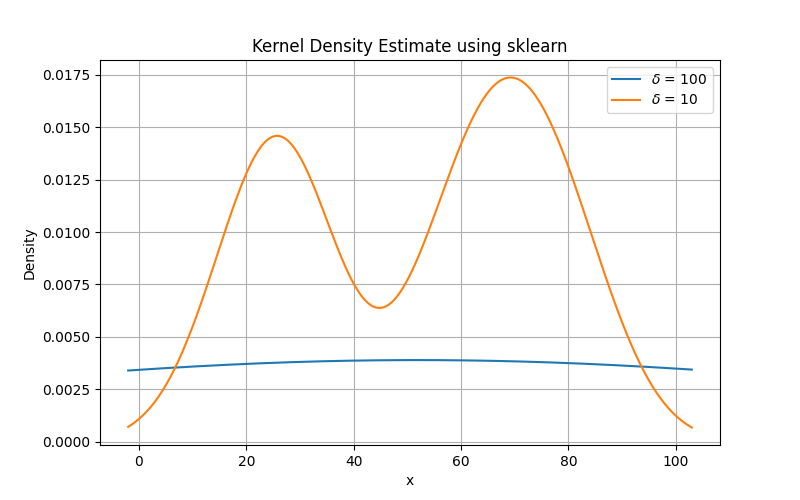
\includegraphics[width=\linewidth]{img/sklearn_kde.png}
        \caption{Computed by the \texttt{sklearn} library}
        \label{fig:subfig1}
    \end{subfigure}%
    \begin{subfigure}{0.5\textwidth}
        \centering
        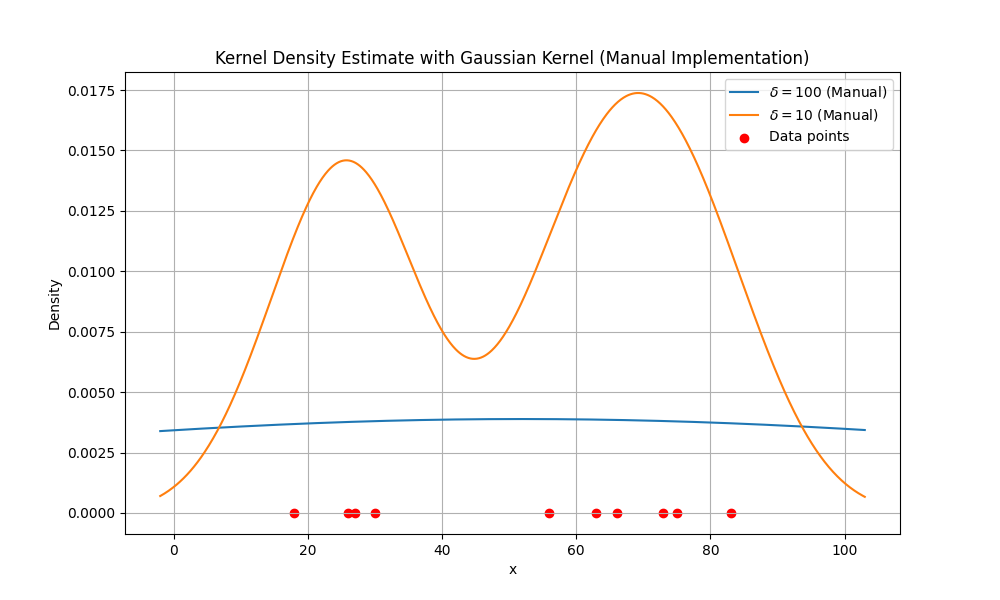
\includegraphics[width=\linewidth]{img/manual_kde.png}
        \caption{Computed via manual implementation}
        \label{fig:subfig2}
    \end{subfigure}
    \caption{KDE with bandwidth parameters \( \delta = 100 \) and \( \delta = 10 \)}
    \label{fig:kde_plot}
\end{figure}

\subsubsection*{Part (b) Compare the two bandwidths}

The choice of $\delta = 10$ is a preferable choice for this dataset, as justified in the following reasons:

\begin{itemize}
    \item Bandwidth $\delta = 10$: The curve is more wiggly and appears to fit closely to the data. It captures the individual peaks in the data distribution, which may indicate local variations in the data.
    \item Bandwidth $\delta = 100$: This curve is smoother and provides a broad overview of the data. It essentially averages out the local variations and might be oversimplifying the data distribution.
\end{itemize}

Method for choosing $\delta$:

\begin{itemize}
    \item \textbf{Cross-Validation}: We can partition the data into training and validation sets, compute the KDE for the training set using a given bandwidth, and then evaluate how well this KDE predicts the validation set. The bandwidth that performs best (typically measured by log-likelihood) on the validation set is chosen.
    \item \textbf{Visual Inspection}: As demonstrated here, a visual inspection of the KDE plot for different bandwidths can give a good idea of which bandwidth provides a better representation of the data.
\end{itemize}

\subsubsection*{Part (c) Probability of new points}

The code in Listing~\ref{code:kde_newpoints} is used  to compute the density \( \tilde{p}(x) \) at the new samples \(x = 30\) and \(x = 95\) for both \( \delta = 100 \) and \( \delta = 10 \).

\begin{listing}[H]
\caption{Calculate the probability of two new samples \(x = 30\) and \(x = 95\)}
\label{code:kde_newpoints}
\begin{minted}[bgcolor=codebg, frame=lines, framesep=2mm, linenos]{python}
# New samples
new_samples = np.array([30, 95]).reshape(-1, 1)

# Calculate densities using sklearn
densities_sklearn = {}
for bandwidth in bandwidths:
    kde = KernelDensity(kernel='gaussian', bandwidth=bandwidth).fit(data)
    log_dens = kde.score_samples(new_samples)
    densities_sklearn[bandwidth] = np.exp(log_dens)

# Calculate densities manually
densities_manual = {}
for bandwidth in bandwidths:
    densities = kde_manual(new_samples.flatten(), data.flatten(), bandwidth)
    densities_manual[bandwidth] = densities

densities_sklearn, densities_manual

# ({100: array([0.00380071, 0.00355839]), 10: array([0.01358759, 0.00292187])},
# {100: array([0.00380071, 0.00355839]), 10: array([0.01358759, 0.00292187])})
\end{minted}
\end{listing}

The densities \( \tilde{p}(x) \) at the new samples \(x = 30\) and \(x = 95\) were calculated both using \texttt{sklearn} and manually, yielding consistent results. The results are as follows:

\begin{itemize}
    \item For \( \delta = 100 \):
    \[\tilde{p}(30) \approx 0.003801, \tilde{p}(95) \approx 0.003558\]
    \item For \( \delta = 10 \):
    \[\tilde{p}(30) \approx 0.013588, \tilde{p}(95) \approx 0.002922\]
\end{itemize}

Furthermore, we use the code in Listing~\ref{code:kde_newpoints_vis} to visualize these new points on the previous plots, as shown in Figure~\ref{fig:kde_newsamples_vis}.  The KDE are displayed with the new samples \(x = 30\) and \(x = 95\) highlighted as red dots for bandwidth parameters \( \delta = 100 \) and \( \delta = 10 \).

\begin{listing}[H]
\caption{Visualize the new samples in the previous KDE plots}
\label{code:kde_newpoints_vis}
\begin{minted}[bgcolor=codebg, frame=lines, framesep=2mm, linenos]{python}
# Function to plot KDE with new samples highlighted
def plot_kde_with_samples(bandwidths, x_vals, data, new_samples, densities_sklearn):
    plt.figure(figsize=(10, 5))
    for bandwidth in bandwidths:
        # Plotting KDE
        densities = kde_manual(x_vals.flatten(), data.flatten(), bandwidth)
        plt.plot(x_vals, densities, label=f'$\delta$ = {bandwidth}')
        
        # Highlighting new samples
        for sample, density in zip(
            new_samples.flatten(), 
            densities_sklearn[bandwidth]
        ):
            plt.plot(sample, density, 'ro')  # red dot for new samples
    
    plt.title('Kernel Density Estimate with New Samples Highlighted')
    plt.legend()
    plt.xlabel('x')
    plt.ylabel('Density')
    plt.grid(True)
    plt.savefig(IMG_PATH + 'kde_with_samples.png')
    plt.show()

# Plotting
plot_kde_with_samples(bandwidths, x_vals, data, new_samples, densities_sklearn)
\end{minted}
\end{listing}

\begin{figure}
    \centering
    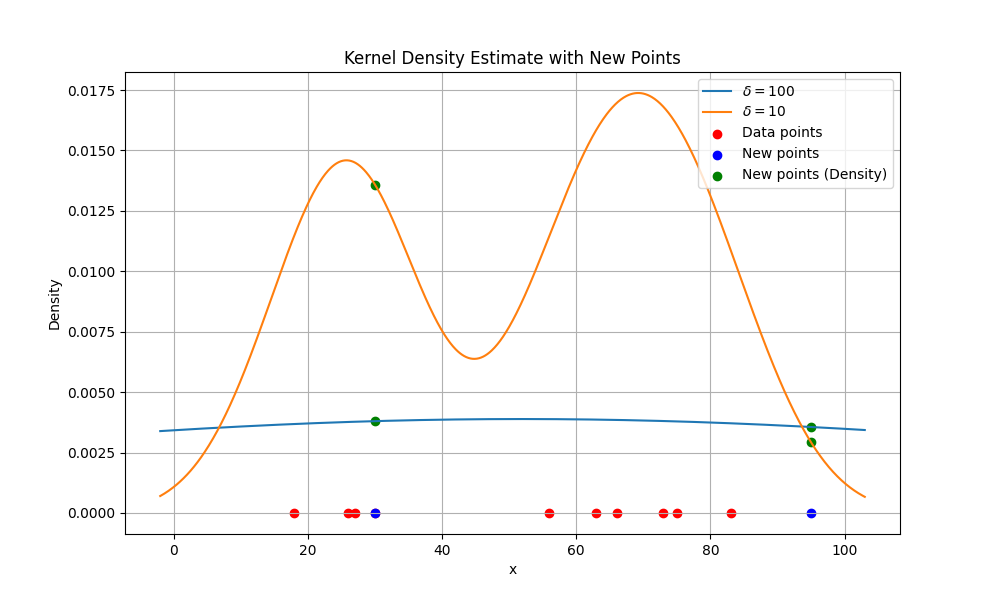
\includegraphics[width=0.8\linewidth]{img/kde_with_samples.png}
    \caption{KDE with new samples highlighted}
    \label{fig:kde_newsamples_vis}
\end{figure}

\subsubsection*{Part (d) Rule to accept or reject points }

A possible rule to determine whether a point is an outlier based on KDE is by setting a threshold density value, \( \tau \). A point \( x \) is considered part of the data distribution if its density \( \tilde{p}(x) \) is above the threshold:

\[
\tilde{p}(x) > \tau
\]

Otherwise, it is considered an outlier. 

However, this strategy might not always work effectively, especially when the data distribution is multi-modal or has varying densities in different regions. In such cases, a global threshold might not suitably differentiate between typical points and outliers. Additionally, the choice of kernel and bandwidth also influences the KDE, making the rule sensitive to these hyperparameters.

\subsubsection*{Compare Gaussian and Tophat kernels}

The code in Listing~\ref{code:kde_tophat} change the kernel to a Tophat kernel and plot the KDE for \( \delta = 10 \). The Tophat kernel is defined as:

\[
K(x, z; \delta) = 
\begin{cases} 
1 & \text{if } \|x-z\| \leq \frac{\delta}{2} \\
0 & \text{otherwise}
\end{cases}
\]

Figure~\ref{fig:kde_tophat} visualizes the kernel density estimate (KDE) using the Tophat kernel with a bandwidth parameter \( \delta = 10 \).

One shortcoming of using the Tophat kernel for outlier detection compared to the Gaussian kernel is its abrupt transition at the boundaries of the kernel window. This can lead to a less smooth and less generalized estimate of the data distribution, making it harder to differentiate between typical points and outliers effectively.

Let's consider a one-dimensional dataset mostly distributed between values \(10\) and \(20\) with a single outlier at value \(35\). 

\begin{itemize}
    \item \textbf{Tophat Kernel}: For a Tophat kernel with a bandwidth parameter, \(\delta = 20\). the outlier might not be effectively identified as the KDE might be influenced heavily due to the uniform weighting within the kernel window.
    \item \textbf{Gaussian Kernel}: For a Gaussian kernel, even if the kernel window includes the outlier, it would assign a lower weight to it due to the decreasing weight assigned to points as they move away from the center of the kernel. In other words, the Gaussian kernel, with its smooth weight transition, can more effectively identify the outlier by assigning lower weights to distant points.
\end{itemize}

\begin{figure}
    \centering
    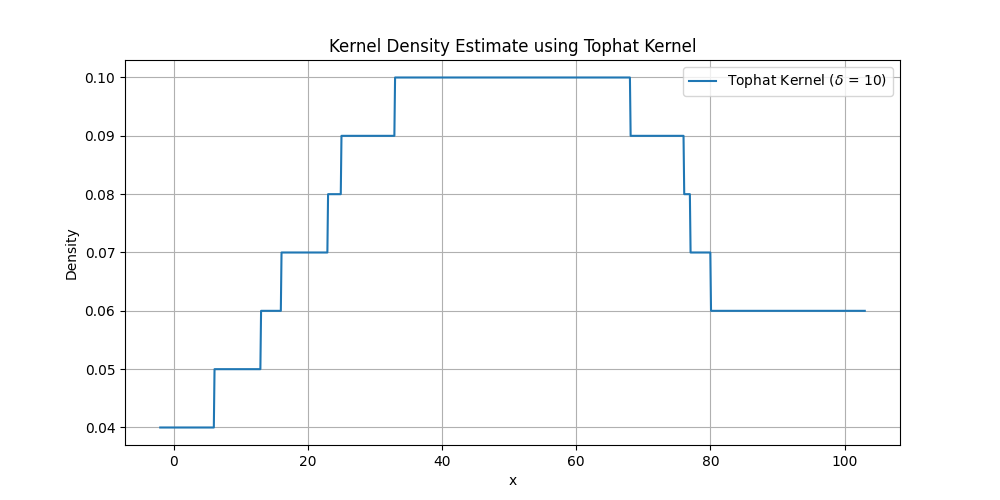
\includegraphics[width=0.8\linewidth]{img/tophat_kde.png}
    \caption{KDE using Tophat Kernal with  \(\delta = 10\)}
    \label{fig:kde_tophat}
\end{figure}

\begin{listing}[H]
\caption{Plot the Tophat density estimate of the dataset using  \(\delta = 10 \) }
\label{code:kde_tophat}
\begin{minted}[bgcolor=codebg, frame=lines, framesep=2mm, linenos]{python}
# Defining the Tophat kernel function
def tophat_kernel(u, delta):
    return 1 if abs(u) <= delta/2 else 0

# Implementing KDE with Tophat kernel
def kde_tophat(x_vals, data, bandwidth):
    densities = []
    for x in x_vals:
        sum_kernel = 0
        for xi in data:
            u = (x - xi) / bandwidth
            sum_kernel += tophat_kernel(u, bandwidth)
        density = (1 / (len(data) * bandwidth)) * sum_kernel
        densities.append(density)
    return np.array(densities)

# Bandwidth for Tophat kernel
bandwidth_tophat = 10

# Plotting the KDE with Tophat kernel
densities_tophat = kde_tophat(x_vals.flatten(), data.flatten(), bandwidth_tophat)
plt.figure(figsize=(10, 5))
plt.plot(x_vals, densities_tophat, 
    label=f'Tophat Kernel ($\delta$ = {bandwidth_tophat})')
plt.title('Kernel Density Estimate using Tophat Kernel')
plt.legend()
plt.xlabel('x')
plt.ylabel('Density')
plt.grid(True)
plt.show()
\end{minted}
\end{listing}



\section{Written Exercises}

\subsection{K-means clustering}

\subsubsection*{Part (a) \(\ J(c_{t-1}, f_t) \le J(c_{t-1}, f_{t-1})\)}

\begin{proof}
Consider a single cluster, denoted by the index \(k\), and let the points in this cluster be given by \(\{x^{(i)}: f_t(x^{(i)}) = k\}\). The objective is to show that the updated centroid, \(c_t^{(k)}\), which is the mean of the points in cluster \(k\), minimizes the sum of squared Euclidean distances to the points in the cluster. Let us denote this sum as \(M_k(c)\), which is formulated as follows:

\[ M_k(c) = \sum_{i:f_t(x^{(i)}) = k} ||x^{(i)} - c||_2^2 \]

To find the value of \(c\) that minimizes \(M_k(c)\), we take the derivative with respect to \(c\) and set it to zero:

\[ \frac{dM_k(c)}{dc} = -2 \sum_{i:f_t(x^{(i)}) = k} (x^{(i)} - c) \]

Solving the equation \(\frac{dM_k(c)}{dc} = 0\), we get:

\[ \sum_{i:f_t(x^{(i)}) = k} (x^{(i)} - c) = 0 \]
\[ \sum_{i:f_t(x^{(i)}) = k} x^{(i)} = c S^{(k)} \]
\[ c = \frac{1}{S^{(k)}} \sum_{i:f_t(x^{(i)}) = k} x^{(i)} \]
\[ c = c_t^{(k)} \]

This confirms that the value of \(c\) which minimizes \(M_k(c)\) is indeed the updated centroid \(c_t^{(k)}\). Consequently, updating the centroids in this manner ensures that the objective function \(J(c_t, f_t)\), which is the sum of Euclidean distances to the points in the cluster, is also minimized, establishing that:

\[ J(c_t, f_t) \leq J(c_{t-1}, f_t) \]
\end{proof}

\subsubsection*{Part (b): \(J(c_t, f_t) \leq J(c_{t-1}, f_t)\)}

\begin{proof}
Consider a single cluster, denoted by the index \(k\), and let the points in this cluster be given by \(\{x^{(i)}: f_t(x^{(i)}) = k\}\). The objective is to show that the updated centroid, \(c_t^{(k)}\), which is the mean of the points in cluster \(k\), minimizes the sum of squared Euclidean distances to the points in the cluster. Let us denote this sum as \(M_k(c)\), which is formulated as follows:

\[ M_k(c) = \sum_{i:f_t(x^{(i)}) = k} ||x^{(i)} - c||_2^2 \]

To find the value of \(c\) that minimizes \(M_k(c)\), we take the derivative with respect to \(c\) and set it to zero:

\[ \frac{dM_k(c)}{dc} = -2 \sum_{i:f_t(x^{(i)}) = k} (x^{(i)} - c) \]

Solving the equation \(\frac{dM_k(c)}{dc} = 0\), we get:

\[ \sum_{i:f_t(x^{(i)}) = k} (x^{(i)} - c) = 0 \]
\[ \sum_{i:f_t(x^{(i)}) = k} x^{(i)} = c S^{(k)} \]
\[ c = \frac{1}{S^{(k)}} \sum_{i:f_t(x^{(i)}) = k} x^{(i)} \]
\[ c = c_t^{(k)} \]

This confirms that the value of \(c\) which minimizes \(M_k(c)\) is indeed the updated centroid \(c_t^{(k)}\). Consequently, updating the centroids in this manner also ensures that the objective function \(J(c_t, f_t)\) is minimized, since it is the sum of Euclidean distances, establishing that:

\[ J(c_t, f_t) \leq J(c_{t-1}, f_t) \]
\end{proof}


\subsection{Local Optima in K-means}

Consider a dataset with the following 1D points:
\[ [0, 2, 6, 11, 12, 13] \]
We want to partition these points into two clusters ($K=2$).

\textbf{Initialization 1:} Centroids: $C_1: 2$, $C_2: 12$

\begin{align*}
\text{Iteration 1:} & \quad 
    \begin{cases} 
    \text{Points closer to } C_1: [0, 2, 6] \\
    \text{Points closer to } C_2: [11, 12, 13] 
    \end{cases} \\
& \quad \text{New centroids: } 
    C_1: \frac{0+2+6}{3} = 2.67, \, 
    C_2: \frac{11+12+13}{3} = 12\\
\text{Iteration 2:} & \quad 
    \begin{cases} 
    \text{Points closer to } C_1: [0, 2, 6] \\
    \text{Points closer to } C_2: [11, 12, 13] 
    \end{cases} \\
& \quad \text{New centroids: } 
    C_1: \frac{0+2+6}{3} = 2.67, \, 
    C_2: \frac{11+12+13}{3} = 12\\
& \text{Stop the iteration here because the centroids do not change anymore.}
\end{align*}

\textbf{Initialization 2:} Centroids: $C_1: 0$, $C_2: 6$

\begin{align*}
\text{Iteration 1:} & \quad 
    \begin{cases} 
    \text{Points closer to } C_1: [0, 2] \\
    \text{Points closer to } C_2: [6, 11, 12, 13] 
    \end{cases} \\
& \quad \text{New centroids: } 
    C_1: \frac{0+2}{2} = 1, \, 
    C_2: \frac{6+11+12+13}{4} = 10.5\\
\text{Iteration 2:} & \quad 
    \begin{cases} 
    \text{Points closer to } C_1: [0, 2] \\
    \text{Points closer to } C_2: [6, 11, 12, 13] 
    \end{cases} \\
& \quad \text{New centroids: } 
    C_1: \frac{0+2}{2} = 1, \, 
    C_2: \frac{6+11+12+13}{4} = 10.5 \\
& \text{Stop the iteration here because the centroids do not change anymore.}
\end{align*}

In \textbf{Initialization 1}, the final clusters are $[0, 2, 6]$ and $[11, 12, 13]$. In \textbf{Initialization 2}, the final clusters are $[0, 2]$ and $[6, 11, 12, 13]$, showcasing the sensitivity of K-means to initial centroid choices.


\end{document}